\documentclass{article}
\usepackage{amsmath, amssymb}
\usepackage{graphicx}
\usepackage{enumerate}
\usepackage{tabularx}
\usepackage{array}
\usepackage{microtype}
\usepackage{booktabs}
\usepackage{cancel}
\usepackage{tikz}
\usepackage{pgfplots}

\newcommand{\tallyV}{$\cancel{||||}$}

\begin{document}

\title{Homework}
\date{Data Analysis}
\author{Preliminary Mathematics Standard}
\maketitle


\section{Questions}
\subsection{Descriptive Statistics}
\begin{enumerate}
 \item A survey was conducted asking members of the public to nominate their preferred sport. The results recorded were:
\begin{center}
\textit{football, cricket, cricket, tennis, basketball, netball, tennis, netball, swimming, netball, tennis, football, cricket, basketball, lawn bowls, football, swimming, netball, tennis, netball, cricket, tennis, football, basketball, swimming, lawn bowls, swimming, swimming, netball, netball, tennis, golf, football, football, basketball, swimming, golf, football, netball, swimming, basketball, basketball, golf, tennis, cricket, cricket, football, basketball, netball, golf.}
\end{center}
 
\begin{enumerate}[(a)]
  \item Is the data collected in this survey an example of numerical or categorical data?
  \item What problems arise when the results of surveys are presented as they are above instead of in table form?
  \item Present the data in a frequency table and use the table to write a description summarising the survey results.
\end{enumerate}

\item \begin{enumerate}[(a)] 
\item List two examples of your own that would be considered discrete data.
\item List two examples of your own that would be considered continuous data.
 \end{enumerate}

\item Students from a Year 11 class were asked about their favourite subjects and the following data was recorded.
\begin{table}[h]
    \centering
    \begin{tabular}{|l|l|l|l|l|}
        \hline
        Maths   & English & PE       & Science & PE       \\ \hline
        Art     & Maths   & Science  & English & Science  \\ \hline
        Cooking & PE      & English  & Cooking & Maths    \\ \hline
        PE      & Art     & Science  & Maths   & Art      \\ \hline
        Science & Cooking & Art      & PE      & PE       \\ \hline
    \end{tabular}
\end{table}
\begin{enumerate}[(a)]
    \item Put the data in a frequency table and record the number of students who were surveyed.
   \item 
What percentage of students preferred Maths?
   \item 
What was the most popular subject? What percentage of students preferred this?
   \item 
What type of data is this?
\end{enumerate}

\item The following Pareto chart shows the causes of home injuries for which children aged 0 to 4 years required hospital treatment in April 2017.
 
\begin{figure}[h]
    \centering
    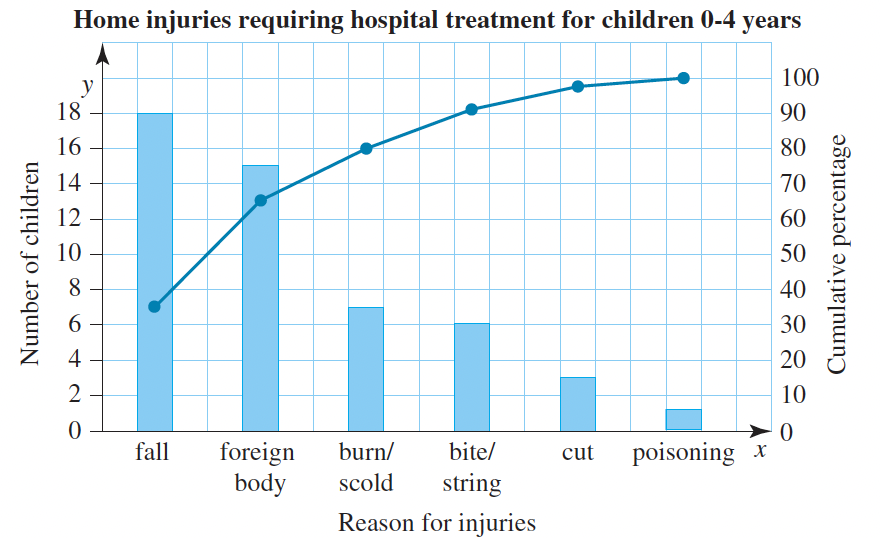
\includegraphics[width=1\linewidth]{Screenshot 2026-04-19 at 10.14.56 am.png}
\end{figure}
 
\begin{enumerate}[(a)]
  \item How many children required hospital treatment in April 2017 for home injuries?
  \item Which reason for home injury for children aged 0 to 4 years is the biggest concern?
  \item What is the cumulative percentage frequency value for burn/scald injuries?
\end{enumerate}
\end{enumerate}

\subsection{Histograms \& Polygons}
\begin{enumerate}
    \item An online bed and breakfast company gives customers the opportunity to review online the bed and
breakfast places that they stayed in. The table and Pareto chart below show the complaints of customers staying at a particular bed and breakfast place located in an alpine resort area.
\begin{table}[h]
    \centering
    \begin{tabular}{l|r}
        \textbf{Customer reasons} & \textbf{Frequency} \\
        \hline
                \hline
        Too cold & 58 \\
        Damp smell & 50 \\
        Old bed linen & 26 \\
        Poor TV reception & 20 \\
        Insuffcient hot water & 18 \\
        Towels too small/thin & 13 \\
        Dated furniture & 8 \\
        Cockroaches & 5 \\
        Inadequate lighting & 2 \\
    \end{tabular}
\end{table}
\begin{figure}[h]
    \centering
    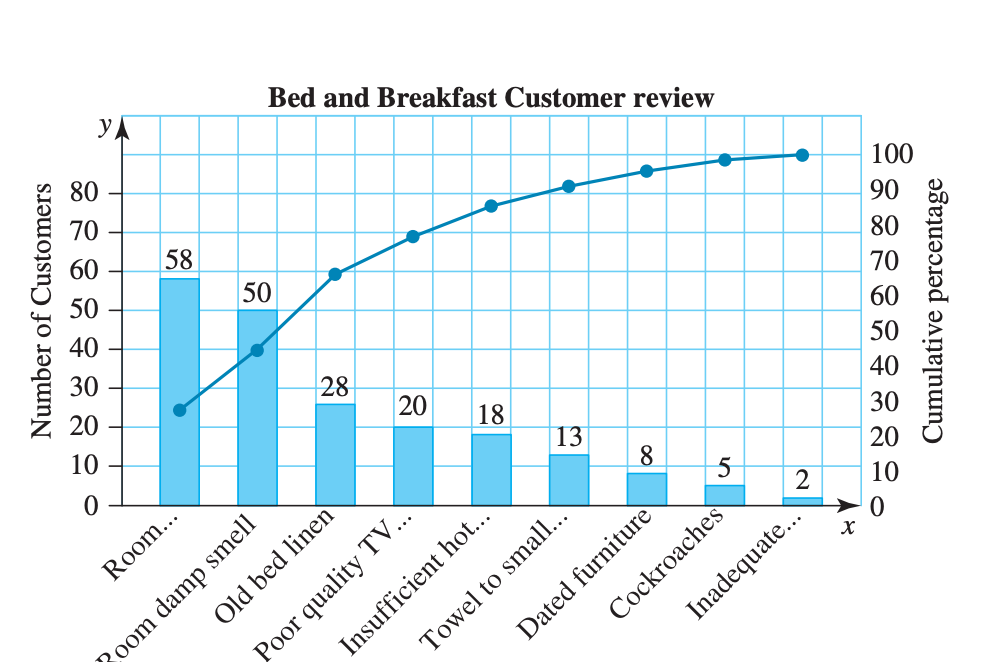
\includegraphics[width=1\linewidth]{brave_screenshot.png}
\end{figure}
\begin{enumerate}[(a)]
    \item How many customers reviewed the bed and breakfast place?
    \item Which reason for customer complaints is the biggest concern for the bed and breakfast?
    \item Is this sampling method used by the online bed and breakfast company biased? Explain. 
\end{enumerate}
\item The following diagram is the result of a student’s attempt to draw a
dot plot to display the values
\begin{center}
    8, 10, 10, 11, 11, 12, 12, 15, 15, 15, 15, 17, 18, 19. 
\end{center}
\begin{figure}[h]
    \centering
    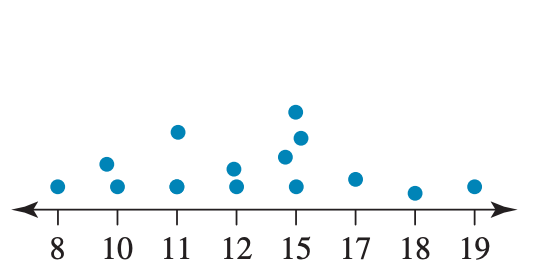
\includegraphics[width=0.5\linewidth]{image.png}
\end{figure}
\begin{enumerate}[(a)]
    \item List the mistakes that the student made in drawing the dot plot.
    \item Draw the correct dot plot. 
\end{enumerate}
\item The maximum daily temperatures (°C) in Sydney
for the month of February were recorded as
follows:
\begin{center}
    28, 24, 29, 37, 35, 30, 31, 27, 34, 29, 25, 36, 36, 37,
36, 30, 42, 41, 42, 41, 38, 37, 33, 27, 26, 36, 27, 26.
\end{center}
\begin{enumerate}[(a)]
    \item Draw a dot plot to display the data.
    \item Comment on the distribution of the data. 
\end{enumerate}
\item Train timetables at railway stations are often presented in a
format similar to stem-and-leaf plots. A section of a timetable
is displayed below.
\begin{table}[h]
    \centering
    \caption{Departure times from Flinders Street station}
    \begin{tabular}{l|l}
        \textit{am} & \\
        6 & 03 23 43 \\
        7 & 03 18 33 48 \\
        8 & 03 10 18 25 33 43 50 \\
        9 & 03 18 33 48\\
    \end{tabular}
\end{table}
\begin{enumerate}[(a)]
    \item What does this timetable use as the stem and the leaf?
    \item  If you arrive at the station at 8:20, what train will
you take?
    \item What beneft does a timetable in this form have compared
with a timetable that lists the full time for each departure? 
\end{enumerate}
\item  Data was collected on the number of times people go
to the cinema in a month.
\begin{center}
    4, 5, 7, 9, 1, 2, 5, 2, 4, 8, 3, 6,\\
2, 3, 8, 1, 1, 4, 5, 3, 3, 6, 1, 2,\\
7, 1, 3, 2, 2, 4, 10, 0, 1, 3, 4,6 \\
\end{center}
\begin{enumerate}[(a)]
    \item  Put the data in a frequency table.
    \item Draw a histogram to represent the data.
    \item How many people go to the cinema less than three
times a month?
    \item  How many people go to the cinema at least three
times a month? 
\end{enumerate}
\item The daily numbers of hits a fashion blogger gets on her new website over 3 weeks are:
\begin{center}
    126 356 408 404 420 425 176\\
167 398 433 446 419 431 189\\
120 431 390 495 454 215 11z
\end{center}
At the same time, the daily number of hits a healthy lifestyle blogger gets on his new website over
3 weeks are:
\begin{center}
    240 156 462 510 420 474 520\\
225 402 426 563 621 339 195\\
320 621 340 495 700 415 371
\end{center}
\begin{enumerate}[(a)]
    \item  Compare the two data sets using an appropriate graphical display.
\item  Comment on the two data sets. 
\end{enumerate}
\item A side-by-side bar chart shows the distributions of New South Wales road fatalities from March 2016
to March 2017. 
\begin{figure}[h]
    \centering
    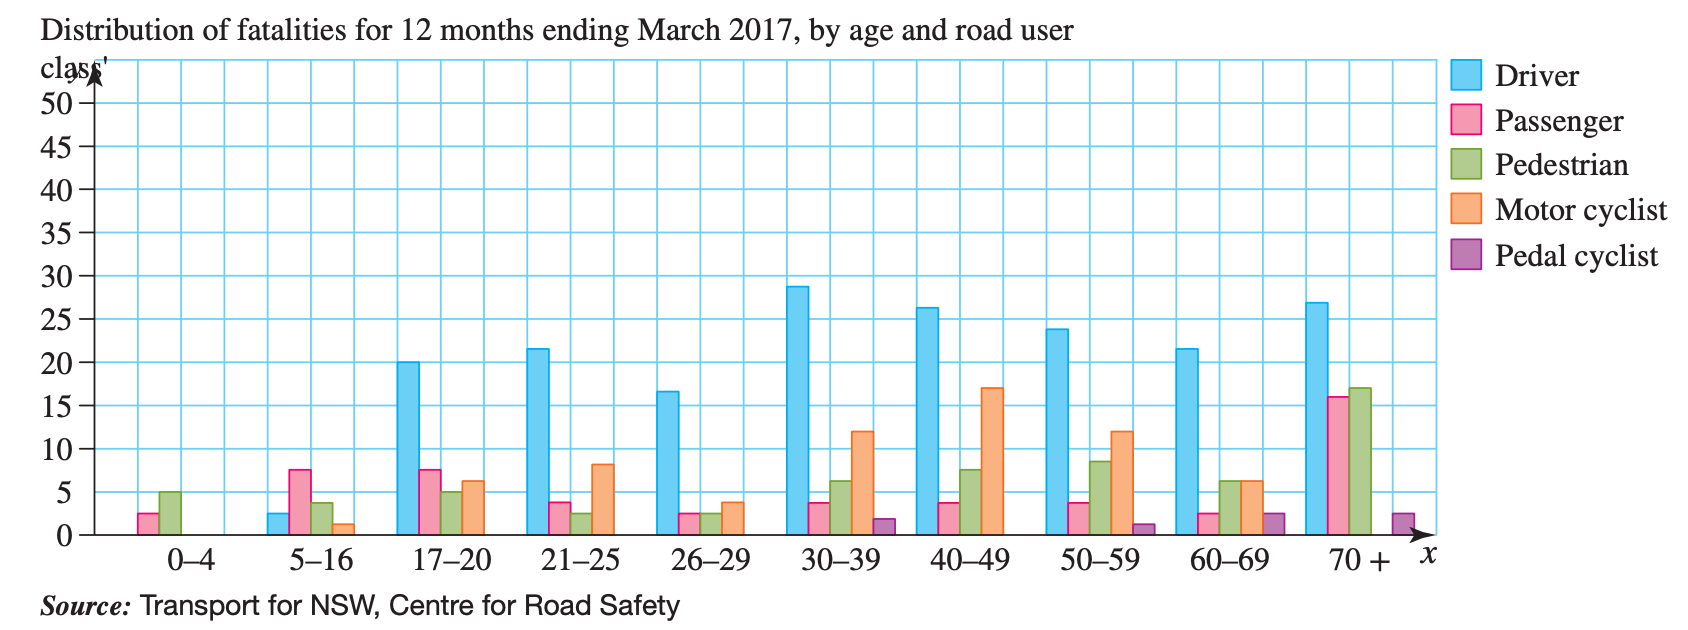
\includegraphics[width=1\linewidth]{image1.png}
\end{figure}
\begin{enumerate}[(a)]
    \item Which age group had the most passenger and pedestrian fatalities? Give a reason why this might be.
    \item The New South Wales government wants to introduce a road campaign. Which age groups should the
government focus on? Explain your answer. 
\end{enumerate}
\item A horizontal side-by-side bar chart shows a monthly comparison of the New South Wales road fatalities.
\begin{figure}[h]
    \centering
    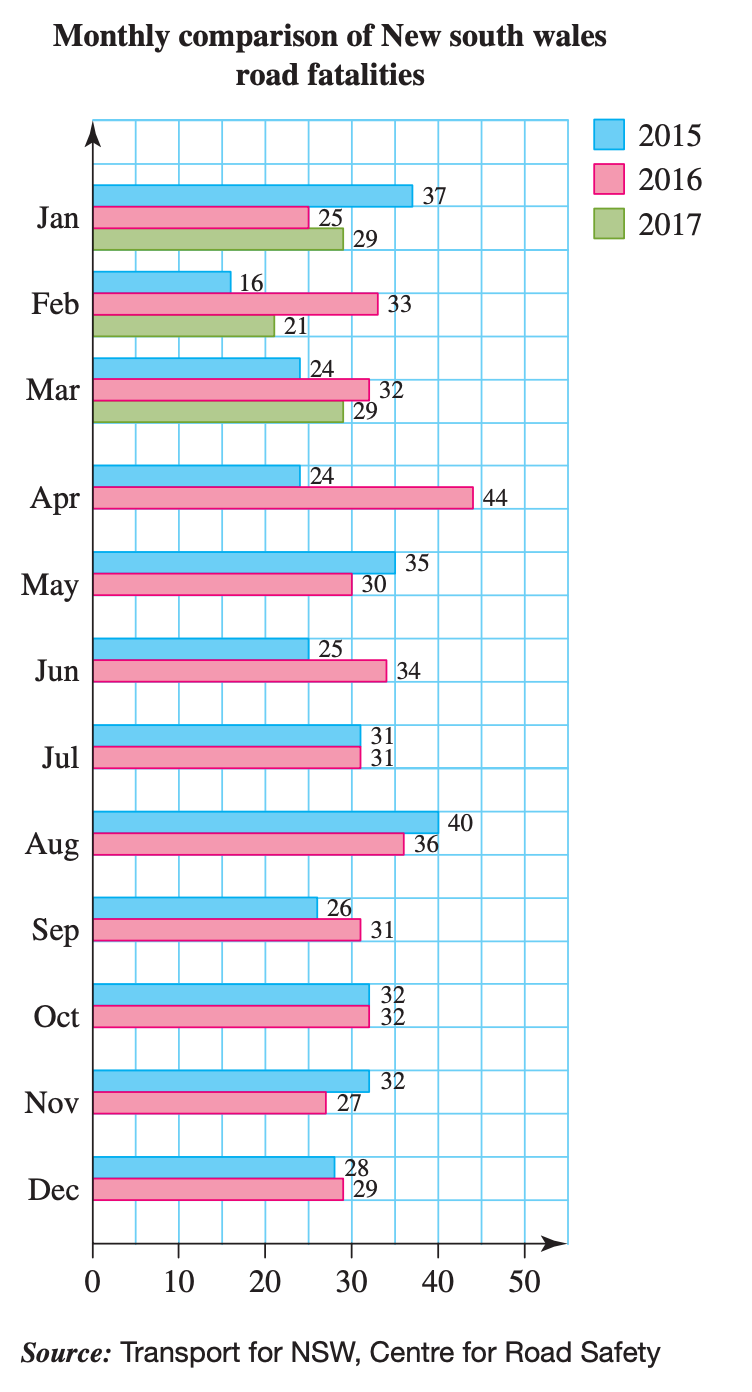
\includegraphics[width=0.5\linewidth]{image2.png}
\end{figure}
\begin{enumerate}[(a)]
    \item Using the data from 2015 and 2016, which year had
the most fatalities on New South Wales roads?
   \item Which year has had the most fatalities from January
to March? 
   \item Why do you think there were 44 fatalities in the
month of April 2016?
\end{enumerate}
\end{enumerate}

\subsection{Measures of Centre and Spread}
\begin{enumerate}

  \item The ages of 9 employees at a small business are:
  \[
    24,\ 31,\ 28,\ 45,\ 31,\ 52,\ 28,\ 31,\ 38
  \]
  \begin{enumerate}[(a)]
    \item Calculate the mean age.
    \item Find the median age.
    \item State the mode.
    \item Calculate the range.
  \end{enumerate}

  \item The following frequency table shows the number of hours per week students spend on social media.
  \begin{center}
    \begin{tabular}{cc}
      \toprule
      \textbf{Hours per week} & \textbf{Frequency} \\
      \midrule
      5  & 4  \\
      10 & 9  \\
      15 & 12 \\
      20 & 7  \\
      25 & 3  \\
      \bottomrule
    \end{tabular}
  \end{center}
  \begin{enumerate}[(a)]
    \item How many students were surveyed?
    \item Calculate the mean number of hours spent on social media per week.
    \item Find the modal number of hours.
    \item Find the median number of hours.
  \end{enumerate}

  \item Two basketball players record their points scored over 8 games:
  \begin{center}
    \textbf{Player A:} $12,\ 15,\ 14,\ 13,\ 16,\ 12,\ 15,\ 11$ \\[4pt]
    \textbf{Player B:} $8,\ 22,\ 10,\ 25,\ 6,\ 19,\ 14,\ 24$
  \end{center}
  \begin{enumerate}[(a)]
    \item Calculate the mean score for each player.
    \item Calculate the range for each player.
    \item Calculate the population standard deviation for each player, correct to 2 decimal places.
    \item Which player would you select for a team that needs a \textit{consistent} scorer? Justify your answer.
  \end{enumerate}

  \item A dataset has a mean of 18, a median of 14 and a mode of 11.
  \begin{enumerate}[(a)]
    \item Which measure of centre would best represent the typical value in this dataset? Justify your answer.
    \item Suggest a possible reason why the mean is so much higher than the median and mode.
    \item Give a real-world context where this pattern of mean $>$ median $>$ mode commonly occurs.
  \end{enumerate}

  \item The daily maximum temperatures (in $^\circ$C) recorded over two weeks in Sydney were:
  \[
    28,\ 31,\ 33,\ 29,\ 35,\ 30,\ 27,\ 26,\ 32,\ 34,\ 31,\ 29,\ 33,\ 30
  \]
  \begin{enumerate}[(a)]
    \item Calculate the mean temperature, correct to 1 decimal place.
    \item Find the median temperature.
    \item Calculate the range.
    \item Calculate the population standard deviation, correct to 2 decimal places.
    \item Describe the distribution shape of this dataset.
  \end{enumerate}

  \item A factory produces bolts. A quality control officer measures the diameter (mm) of a sample of 10 bolts:
  \[
    10.1,\ 10.3,\ 9.8,\ 10.2,\ 10.0,\ 10.4,\ 9.9,\ 10.1,\ 10.2,\ 10.0
  \]
  \begin{enumerate}[(a)]
    \item Calculate the mean diameter.
    \item Calculate the population standard deviation, correct to 3 decimal places.
    \item A second machine produces bolts with a mean diameter of $10.1$ mm and a standard deviation of $0.25$ mm. Which machine produces more consistent bolts? Justify your answer.
    \item Why is consistency important in manufacturing? 
  \end{enumerate}

  \item The stem-and-leaf plot below shows the marks (out of 50) scored by students on a test.
  \begin{center}
    \begin{tabular}{r|l}
      \textbf{Stem} & \textbf{Leaf} \\
      \hline
      2 & 3\ \ 5\ \ 8 \\
      3 & 1\ \ 1\ \ 4\ \ 7\ \ 9 \\
      4 & 0\ \ 2\ \ 2\ \ 5\ \ 5\ \ 5\ \ 8 \\
      5 & 0\ \ 0 \\
    \end{tabular}
  \end{center}
  \begin{enumerate}[(a)]
    \item How many students sat the test?
    \item Write out the full dataset in order.
    \item Find the median mark.
    \item State the mode.
    \item Calculate the range.
    \item Describe the shape of this distribution.
  \end{enumerate}

  \item The annual salaries of employees at a company are:
  \[
    \$52\,000,\ \$55\,000,\ \$58\,000,\ \$61\,000,\ \$63\,000,\ \$410\,000
  \]
  \begin{enumerate}[(a)]
    \item Calculate the mean salary.
    \item Find the median salary.
    \item A journalist reports that the ``average'' salary at the company is over \$100\,000. Which measure of centre are they using, and is this a fair representation? Explain.
    \item Which measure of centre best represents the typical salary? Why?
  \end{enumerate}

  \item The number of goals scored per match by a soccer team over a season is shown in the table below.
  \begin{center}
    \begin{tabular}{ccc}
      \toprule
      \textbf{Goals scored} & \textbf{Frequency} & \textbf{Cumulative frequency} \\
      \midrule
      0 & 3  & \\
      1 & 7  & \\
      2 & 10 & \\
      3 & 6  & \\
      4 & 4  & \\
      \bottomrule
    \end{tabular}
  \end{center}
  \begin{enumerate}[(a)]
    \item Complete the cumulative frequency column.
    \item How many matches did the team play?
    \item Calculate the mean number of goals per match.
    \item Use the cumulative frequency column to find the median.
    \item State the mode.
    \item Calculate the population standard deviation, correct to 2 decimal places.
  \end{enumerate}

  \item A dataset of 7 values has the following properties:
  \[
    \text{Mean} = 12, \quad \text{Mode} = 10, \quad \text{Range} = 14
  \]
  The dataset contains the values $10,\ 10,\ 8,\ 15,\ 22$ and two unknown values $a$ and $b$, where $a < b$.
  \begin{enumerate}[(a)]
    \item Use the mean to write an equation involving $a$ and $b$.
    \item Use the range to write a second equation or inequality involving $a$ and $b$.
    \item Hence find the values of $a$ and $b$.
    \item Calculate the population standard deviation of the complete dataset, correct to 2 decimal places.
  \end{enumerate}

\end{enumerate}

\subsection{Quartiles, Box Plots and Outliers}
\begin{enumerate}

  \item Find the five-number summary and IQR for the following dataset:
  \[
    4,\ 7,\ 9,\ 12,\ 15,\ 18,\ 21,\ 24,\ 27
  \]

  \item The ages of 10 people at a community event were recorded as:
  \[
    14,\ 19,\ 22,\ 25,\ 25,\ 31,\ 34,\ 38,\ 45,\ 52
  \]
  \begin{enumerate}[(a)]
    \item Find the five-number summary.
    \item Calculate the IQR.
    \item Calculate the range.
    \item Which measure of spread --- range or IQR --- better represents this dataset? Justify
    your answer.
  \end{enumerate}

  \item The dot plot below shows the number of text messages sent by 12 students in one day.
  \begin{center}
  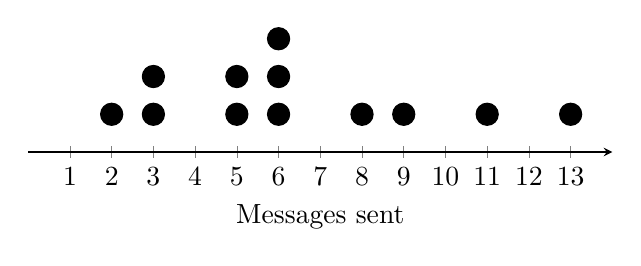
\begin{tikzpicture}
    \begin{axis}[
      axis x line=bottom, axis y line=none,
      xmin=0, xmax=14, ymin=0, ymax=4,
      xtick={1,2,3,4,5,6,7,8,9,10,11,12,13},
      xlabel={Messages sent},
      width=9cm, height=3.5cm,
      clip=false
    ]
      \addplot[only marks, mark=*, mark size=4pt] coordinates {
        (2,1)(3,1)(3,2)(5,1)(5,2)(6,1)(6,2)(6,3)(8,1)(9,1)(11,1)(13,1)
      };
    \end{axis}
  \end{tikzpicture}
  \end{center}
  \begin{enumerate}[(a)]
    \item Write out the dataset in order.
    \item Determine the five-number summary.
    \item Draw a box plot to represent this data.
  \end{enumerate}

  \item The following frequency histogram shows the heights (cm) of 20 students.
  \begin{center}
  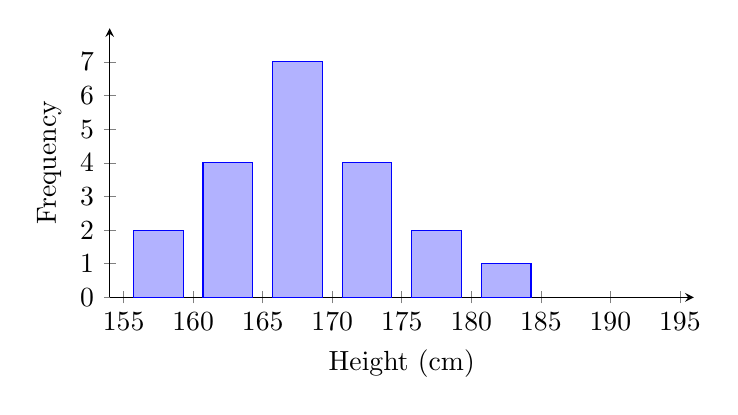
\begin{tikzpicture}
    \begin{axis}[
      ybar, bar width=18pt,
      axis x line=bottom, axis y line=left,
      xmin=154, xmax=196,
      ymin=0, ymax=8,
      xtick={155,160,165,170,175,180,185,190,195},
      ytick={0,1,2,3,4,5,6,7},
      xlabel={Height (cm)},
      ylabel={Frequency},
      width=9cm, height=5cm
    ]
      \addplot coordinates {(157.5,2)(162.5,4)(167.5,7)(172.5,4)(177.5,2)(182.5,1)};
    \end{axis}
  \end{tikzpicture}
  \end{center}
  \begin{enumerate}[(a)]
    \item How many students are in the dataset?
    \item Determine the five-number summary.
    \item Construct a box plot for this data.
    \item Describe the shape of the distribution.
  \end{enumerate}

  \item The following dataset contains an error made during data collection:
  \[
    11,\ 13,\ 14,\ 15,\ 15,\ 16,\ 17,\ 18,\ 82
  \]
  \begin{enumerate}[(a)]
    \item Calculate $Q_1$, $Q_3$ and the IQR.
    \item Use the outlier formula to determine whether 82 is a formal outlier.
    \item Calculate the mean with and without the outlier.
    \item Calculate the median with and without the outlier.
    \item What do your results suggest about the effect of outliers on the mean versus the median?
  \end{enumerate}

  \item The results of a class spelling test (out of 20) are shown below:
  \[
    8,\ 10,\ 11,\ 12,\ 13,\ 13,\ 14,\ 14,\ 15,\ 15,\ 15,\ 16,\ 17,\ 18,\ 19
  \]
  \begin{enumerate}[(a)]
    \item Find the five-number summary.
    \item Draw a box plot to represent this data on a clearly labelled number line.
    \item Identify any clusters or gaps in the data and explain what they might suggest.
    \item Are there any outliers? Show your working using the formal outlier rule.
  \end{enumerate}

  \item Two rugby teams record their points scored across a season. The five-number summaries
  are given below.
  \begin{center}
    \begin{tabular}{lccccc}
      \toprule
      & \textbf{Min} & $Q_1$ & \textbf{Median} & $Q_3$ & \textbf{Max} \\
      \midrule
      Team A & 6  & 14 & 22 & 28 & 38 \\
      Team B & 10 & 18 & 24 & 30 & 44 \\
      \bottomrule
    \end{tabular}
  \end{center}
  \begin{enumerate}[(a)]
    \item Draw a parallel box plot for both teams on the same number line.
    \item Calculate the IQR for each team.
    \item Compare the centres of the two distributions.
    \item Compare the spreads of the two distributions.
    \item Which team is more consistent? Justify your answer.
    \item Describe the shape of each distribution from the box plot.
  \end{enumerate}

  \item The following parallel box plots show the daily maximum temperatures ($^\circ$C) recorded
  in two cities over one month.
  \begin{center}
  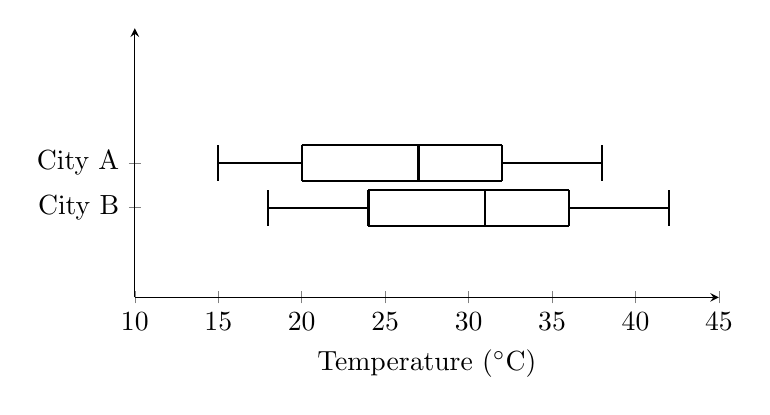
\begin{tikzpicture}
    \begin{axis}[
      width=9cm, height=5cm,
      xmin=10, xmax=45,
      ytick={1,1.5}, yticklabels={City B, City A},
      xlabel={Temperature ($^\circ$C)},
      axis x line=bottom, axis y line=left,
      ymin=0, ymax=3
    ]
      % City A box plot
      \addplot[thick] coordinates {(15,1.3)(15,1.7)};
      \addplot[thick] coordinates {(15,1.5)(20,1.5)};
          \addplot[thick] coordinates {(20,1.3)(20,1.7)};
      \addplot[thick] coordinates {(20,1.3)(32,1.3)};
      \addplot[thick] coordinates {(20,1.7)(32,1.7)};
      \addplot[thick] coordinates {(27,1.3)(27,1.7)};
      \addplot[thick] coordinates {(32,1.3)(32,1.7)};
      \addplot[thick] coordinates {(32,1.5)(38,1.5)};
      \addplot[thick] coordinates {(38,1.3)(38,1.7)};
      % City B box plot
      \addplot[thick] coordinates {(18,0.8)(18,1.2)};
      \addplot[thick] coordinates {(18,1.0)(24,1.0)};
          \addplot[thick] coordinates {(24,0.8)(24,1.2)};
      \addplot[thick] coordinates {(24,0.8)(36,0.8)};
      \addplot[thick] coordinates {(24,1.2)(36,1.2)};
      \addplot[thick] coordinates {(31,0.8)(31,1.2)};
      \addplot[thick] coordinates {(36,0.8)(36,1.2)};
      \addplot[thick] coordinates {(36,1.0)(42,1.0)};
      \addplot[thick] coordinates {(42,0.8)(42,1.2)};
    \end{axis}
  \end{tikzpicture}
  \end{center}
  \begin{enumerate}[(a)]
    \item State the median temperature for each city.
    \item Calculate the IQR for each city.
    \item Which city had a higher typical temperature? Justify using statistics.
    \item Which city had more variable temperatures? Justify your answer.
    \item Compare the shapes of the two distributions.
  \end{enumerate}

  \item A dataset of house prices (\$'000s) in a suburb is:
  \[
    420,\ 445,\ 460,\ 475,\ 480,\ 490,\ 505,\ 510,\ 520,\ 1250
  \]
  \begin{enumerate}[(a)]
    \item Find the five-number summary.
    \item Use the formal outlier rule to determine whether \$1\,250\,000 is an outlier.
    \item Calculate the mean and median with the outlier included.
    \item Calculate the mean and median with the outlier excluded.
    \item A real estate agent advertises the ``average'' house price using the mean including the
    outlier. Is this misleading? Justify your answer.
    \item Which measure of centre is more appropriate here? Why?
  \end{enumerate}

  \item The times (in minutes) taken by 14 runners to complete a 10 km race were:
  \[
    38,\ 41,\ 44,\ 44,\ 46,\ 47,\ 49,\ 51,\ 52,\ 54,\ 55,\ 58,\ 61,\ 90
  \]
  \begin{enumerate}[(a)]
    \item Find the five-number summary.
    \item Formally test whether 90 minutes is an outlier.
    \item Draw a box plot, marking any outliers as separate points.
    \item Describe the shape of the distribution.
    \item Identify any clusters or gaps. Suggest a real-world reason for the outlier.
  \end{enumerate}

  \item The box plot below represents the scores of 30 students on a maths exam.
  \begin{center}
  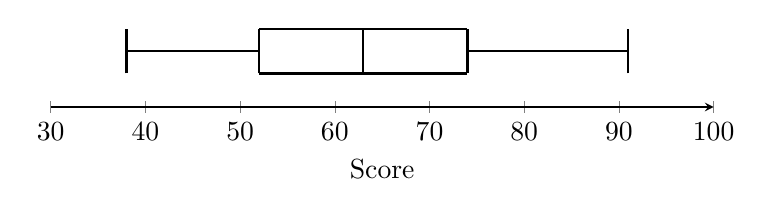
\begin{tikzpicture}
    \begin{axis}[
      width=10cm, height=3cm,
      xmin=30, xmax=100,
      ytick=\empty,
      xlabel={Score},
      axis x line=bottom, axis y line=none,
      ymin=0, ymax=2
    ]
      \addplot[thick] coordinates {(38,0.6)(38,1.4)};
      \addplot[thick] coordinates {(38,1.0)(52,1.0)};
      \addplot[thick] coordinates {(52,0.6)(52,1.4)};

      \addplot[thick] coordinates {(52,0.6)(74,0.6)};
      \addplot[thick] coordinates {(52,1.4)(74,1.4)};
      \addplot[thick] coordinates {(63,0.6)(63,1.4)};
      \addplot[thick] coordinates {(74,0.6)(74,1.4)};
      \addplot[thick] coordinates {(74,1.0)(91,1.0)};
      \addplot[thick] coordinates {(91,0.6)(91,1.4)};
    \end{axis}
  \end{tikzpicture}
  \end{center}
  \begin{enumerate}[(a)]
    \item State the five-number summary.
    \item Calculate the IQR and range.
    \item What percentage of students scored between 52 and 74?
    \item What percentage of students scored above 63?
    \item The pass mark is 50. Estimate the percentage of students who passed.
    \item Describe the shape of the distribution and what it suggests about student performance.
  \end{enumerate}

  \item The number of daily visitors to two websites over 11 days were recorded:
  \begin{center}
    \textbf{Site A:} $120,\ 135,\ 140,\ 142,\ 145,\ 148,\ 150,\ 153,\ 155,\ 160,\ 162$\\[4pt]
    \textbf{Site B:} $80,\ 95,\ 110,\ 130,\ 145,\ 150,\ 155,\ 170,\ 185,\ 200,\ 310$
  \end{center}
  \begin{enumerate}[(a)]
    \item Find the five-number summary for each site.
    \item Calculate the IQR and range for each site.
    \item Formally test whether 310 is an outlier for Site B.
    \item Draw a parallel box plot for both sites, marking any outliers.
    \item Compare the centre, spread and shape of the two distributions.
    \item Which site has more predictable daily traffic? Justify your answer.
  \end{enumerate}

  \item A dataset has the following five-number summary:
  \[
    \text{Min} = 12,\quad Q_1 = 20,\quad Q_2 = 28,\quad Q_3 = 35,\quad \text{Max} = 60
  \]
  \begin{enumerate}[(a)]
    \item Calculate the IQR.
    \item Use the formal outlier rule to find the upper and lower fences.
    \item Is the maximum value of 60 a formal outlier?
    \item Sketch the box plot, marking any outliers appropriately.
    \item Describe the shape of the distribution from the box plot.
    \item Explain how removing the outlier (if any) would affect the mean and standard deviation.
  \end{enumerate}

\end{enumerate}

\subsection{Statistical Investigation Process and Sampling}
\begin{enumerate}

  \item A student wants to investigate the sleeping habits of teenagers in Australia. She
  decides to post a survey on her personal social media page and record the responses.
  \begin{enumerate}[(a)]
    \item What is the population for this investigation?
    \item What sampling method is she using?
    \item Give two reasons why her sample may not be representative of the population.
    \item Rewrite the following survey question to make it clear and unambiguous:\\
    \textit{``Do you sleep enough and wake up feeling okay?''}
    \item The survey asks respondents to select their age group from: ``young, middle-aged,
    old.'' Identify two problems with these response options and suggest an improvement.
  \end{enumerate}

  \item A school of 900 students is divided into three year groups: 300 in Year 10, 360 in
  Year 11 and 240 in Year 12. A researcher wants to take a stratified sample of 90 students.
  \begin{enumerate}[(a)]
    \item Explain why stratified sampling is more appropriate than simple random sampling for
    this investigation.
    \item Calculate how many students should be selected from each year group.
    \item Describe how the researcher would then select the students from each year group.
  \end{enumerate}

  \item For each of the following scenarios, identify the sampling method being used and
  state one advantage and one disadvantage of that method.
  \begin{enumerate}[(a)]
    \item A supermarket surveys every 15th customer who enters the store on a Saturday morning.
    \item A radio station asks listeners to call in and vote on whether a new law should be
    introduced.
    \item A researcher assigns every employee in a company a number and uses a random number
    table to select 40 of them.
    \item A hospital divides its patients into age groups and randomly selects a proportional
    number from each group for a health survey.
  \end{enumerate}

  \item Read the following survey questions and identify the problem with each. Then rewrite
  each question to correct the issue.
  \begin{enumerate}[(a)]
    \item ``Don't you think the government should spend more money on public transport?''
    \item ``How many hours do you spend exercising and cooking healthy meals each week?''
    \item ``Do you sometimes occasionally skip breakfast sometimes?''
    \item ``Rate your income: low / okay / high.''
  \end{enumerate}

  \item A researcher is investigating whether drinking coffee improves study performance in
  university students. She observes students in a library and notes whether they have a coffee
  cup and how long they study for.
  \begin{enumerate}[(a)]
    \item What type of data collection method is being used?
    \item Identify one potential confounding variable in this study.
    \item Explain why the researcher cannot conclude that coffee \textit{causes} students to
    study longer.
    \item Suggest a more controlled method the researcher could use to better investigate this
    question.
  \end{enumerate}

  \item A factory produces 2\,400 phone cases per day. A quality inspector wants to check a
  sample of 80 cases for defects using systematic sampling.
  \begin{enumerate}[(a)]
    \item Calculate the sampling interval.
    \item Describe how the inspector would carry out this sampling method.
    \item Suggest one situation in which systematic sampling could produce a biased sample
    in this context.
    \item If it was found that defective cases tend to occur in groups of 30 during a shift
    change, which sampling method would be more appropriate? Justify your answer.
  \end{enumerate}

  \item Two newspaper headlines report on the same dataset about average weekly wages:
  \begin{center}
    \textbf{Headline A:} \textit{``Average wage rises to \$1\,450 --- workers better off than
    ever!''}\\[6pt]
    \textbf{Headline B:} \textit{``Half of all workers earn less than \$1\,100 a week''}
  \end{center}
  \begin{enumerate}[(a)]
    \item Which measure of centre is Headline A most likely using? Which is Headline B using?
    \item Suggest why the two headlines give such different impressions of the same data.
    \item What does the difference between these two values suggest about the shape of the
    income distribution?
    \item Which headline gives a more accurate picture of the typical worker's wage? Justify
    your answer.
  \end{enumerate}

  \item A local council wants to find out whether residents support the construction of a new
  sports centre. They are considering three data collection approaches:
  \begin{itemize}
    \item \textbf{Option A:} Mail a survey to every 10th household on the electoral roll
    \item \textbf{Option B:} Set up a booth at the shopping centre and invite passers-by to
    respond
    \item \textbf{Option C:} Post a survey link on the council's Facebook page
  \end{itemize}
  \begin{enumerate}[(a)]
    \item Identify the sampling method used in each option.
    \item For each option, describe one way in which the sample may not represent the full
    population of residents.
    \item Which option would produce the most representative sample? Justify your answer.
    \item Suggest one ethical consideration the council should address in any of these surveys.
  \end{enumerate}

  \item A study reports: \textit{``Suburbs with more ice cream shops have higher rates of
  drowning deaths. Therefore, ice cream causes drowning.''}
  \begin{enumerate}[(a)]
    \item Identify the flaw in the study's conclusion.
    \item Suggest a variable that could explain the relationship between ice cream sales and
    drowning rates.
    \item What is the term for a variable that influences both the explanatory and response
    variables in a study?
    \item Give one other real-world example of two variables that are correlated but where
    one does not cause the other.
  \end{enumerate}

  \item A researcher is designing a survey to investigate the dietary habits of Australian
  adults aged 18--65. She plans to survey 200 people.
  \begin{enumerate}[(a)]
    \item Identify one issue of privacy the researcher should consider and explain how she
    could address it.
    \item The researcher plans to conduct the survey only at a gym on weekday mornings.
    Identify two groups of the population who would be underrepresented and explain the impact
    this would have on the results.
    \item Write two survey questions --- one about fruit consumption and one about fast food
    consumption --- that follow good questionnaire design principles. Each question must
    include response options.
    \item The researcher finds that 85\% of respondents eat fruit daily and concludes that
    ``most Australian adults have a healthy diet.'' Identify two problems with this conclusion.
  \end{enumerate}

\end{enumerate}

\newpage
\section{Answers}
\subsection{Descriptive Statistics}
\begin{enumerate}
    \item \begin{enumerate}[(a)]
  \item Categorical
  \item Very difficult to accurately analyse the results
  \item  \phantom{x}
  \vspace{0.4em}
  \begin{center}
  \renewcommand{\arraystretch}{1.4}
  \begin{tabular}{lc}
    \toprule
    \textbf{Sport} & \textbf{Frequency} \\
    \midrule
    Netball    & 9 \\
    Football   & 8 \\
    Tennis     & 7 \\
    Basketball & 7 \\
    Swimming   & 7 \\
    Cricket    & 6 \\
    Golf       & 4 \\
    Lawn bowls & 2 \\
    \bottomrule
  \end{tabular}
  \end{center}
 
  \vspace{0.3em}
  The popularity of most sports was evenly spread, with the exception of the low-scoring lawn bowls and golf.
\end{enumerate}
  
\item Answers will vary. Examples are given.
\begin{enumerate}[(a)] 
  \item Number of people in a cinema; number of security boxes at a bank
  \item Weights of students in your class; distance each student lives from school
\end{enumerate}
 
\item 
\begin{enumerate}[(a)]
  \item \phantom{x}
  \begin{center}
  \renewcommand{\arraystretch}{1.4}
  \begin{tabular}{lcc}
    \toprule
    \textbf{Subject} & \textbf{Tally} & \textbf{Frequency ($f$)} \\
    \midrule
    Maths   & $||||$           & 4  \\
    Art     & $||||$           & 4  \\
    Cooking & $|||$            & 3  \\
    PE      & \tallyV\ $|$     & 6  \\
    Science & \tallyV          & 5  \\
    English & $|||$            & 3  \\
    \midrule
    \textbf{Total} & & \textbf{25} \\
    \bottomrule
  \end{tabular}
  \end{center}
 
 
  \item 16\%
  \item PE; 24\%
  \item Nominal (categorical)
\end{enumerate}
 
\item 
\begin{enumerate}[(a)]
  \item 50
  \item Fall
  \item 80\%
\end{enumerate}
\end{enumerate}

\subsection{Histograms \& Polygons}
\begin{enumerate}
    \item 
\begin{enumerate}[(a)]
    \item 200
    \item Room temperature too cold
    \item Answers will vary. The sampling method used by the bed and breakfast is biased as the online reviews are voluntary.
Guests can submit multiple reviews, and dissatisfed guests are more likely to write a review and give their opinion. 
\end{enumerate}
\item \begin{enumerate}[(a)]
    \item Dots are not aligned vertically. The horizontal scale is not equally sapaced. 
    \item 
\begin{figure}[h]
    \centering
    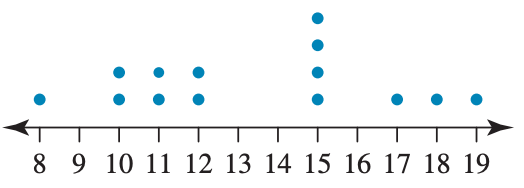
\includegraphics[width=0.5\linewidth]{image3.png}
\end{figure}
\end{enumerate}
\item 12
\begin{enumerate}[(a)]
    \item 
\begin{figure}[h]
        \centering
        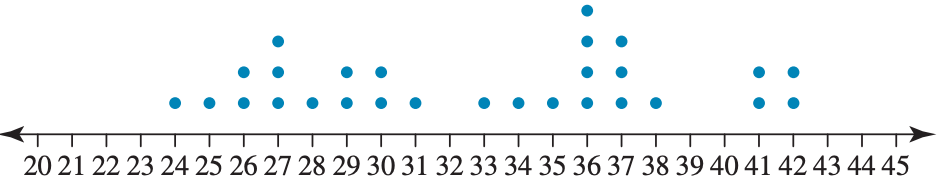
\includegraphics[width=0.75\linewidth]{image4.png}
    \end{figure}
        \item There is a wide spread of temperatures. 
\end{enumerate}
\item 
\begin{enumerate}[(a)]
    \item The stem represents the hour and the leaves represent the minutes.
    \item  8:25 am
    \item This type of timetable enables the viewer to see times at a glance, and it saves space. 
\end{enumerate}
\item  
\begin{enumerate}[(a)]
    \item 
    \item 
    \item 13
    \item  23
\end{enumerate}
\item 
\begin{enumerate}[(a)]
    \item  
\item  Answers will vary. Example answer:
The fashion blogger had 400–<450 hits on her website on 9 days in the 3-week period. The healthy life style blogger got a
wider spread of hits. He received over 400 hits for 11 days in the 3-week period. His website seems to be gaining in
popularity.  
\end{enumerate}
\item 
\begin{enumerate}[(a)]
    \item 70 + age group. Answers about the reason will vary. Elderly people don’t drive as much and tend to walk or be passengers. 
    \item Answers will vary. The road campaign could focus on:
\begin{itemize}
    \item elderly people as pedestrians — being alert when crossing a road.
\item motorcyclists in the 30–49 age group, not on probationary license -- risk taking
\item driving for all age groups — awareness and safety for all drivers. 
\end{itemize}
\end{enumerate}
\item 
\begin{enumerate}[(a)]
    \item 2016
   \item 2016
   \item Answers will vary but could include that more people are on the roads during the Easter break and school holidays. 
\end{enumerate}
\end{enumerate}

\subsection{Measures of Centre and Spread}
\begin{enumerate}
  \item
  \begin{enumerate}[(a)]
    \item Mean $= 34.2$ years
    \item Median $= 31$
    \item Mode $= 31$
    \item Range $= 28$
  \end{enumerate}

  \item
  \begin{enumerate}[(a)]
    \item $n = 35$
    \item Mean $= 14.43$ hours
    \item Mode $= 15$ hours
    \item Median $= 15$ hours
  \end{enumerate}

  \item
  \begin{enumerate}[(a)]
    \item Player A: mean $= 13.5$; Player B: mean $= 16$
    \item Player A: range $= 5$; Player B: range $= 19$
    \item Player A: $\sigma \approx 1.58$; Player B: $\sigma \approx 6.87$
    \item Player A --- lower standard deviation indicates more consistent scoring
  \end{enumerate}

  \item
  \begin{enumerate}[(a)]
    \item Median ($= 14$) --- less affected by the outlier(s) pulling the mean up
  \end{enumerate}

  \item
  \begin{enumerate}[(a)]
    \item Mean $\approx 30.6^\circ$C
    \item Median $= 30.5^\circ$C
    \item Range $= 9^\circ$C
    \item $\sigma \approx 2.37^\circ$C
    \item Approximately unimodal and roughly symmetric
  \end{enumerate}

  \item
  \begin{enumerate}[(a)]
    \item Mean $= 10.1$ mm
    \item $\sigma \approx 0.167$ mm
    \item First machine ($\sigma \approx 0.167$ mm $<$ $0.25$ mm)
  \end{enumerate}

  \item
  \begin{enumerate}[(a)]
    \item $n = 17$
    \item $23, 25, 28, 31, 31, 34, 37, 39, 40, 42, 42, 45, 45, 45, 48, 50, 50$
    \item Median $= 42$
    \item Mode $= 45$
    \item Range $= 27$
    \item Approximately unimodal, slightly negatively skewed
  \end{enumerate}

  \item
  \begin{enumerate}[(a)]
    \item Mean $= \$116\,500$
    \item Median $= \$59\,500$
    \item[(c--d)] Median ($= \$59\,500$) --- the \$410\,000 salary is an outlier that heavily inflates the mean
  \end{enumerate}

  \item
  \begin{enumerate}[(a)]
    \item $3,\ 10,\ 20,\ 26,\ 30$
    \item $n = 30$ matches
    \item Mean $= 2.03$ goals
    \item Median $= 2$ goals
    \item Mode $= 2$ goals
    \item $\sigma \approx 1.13$
  \end{enumerate}

  \item
  \begin{enumerate}[(a)]
    \item $a + b = 19$
    \item $b = 22$ or $b \leq 22$
    \item $a = 6,\ b = 13$
    \item $\sigma \approx 4.27$
  \end{enumerate}

\end{enumerate}

\subsection{Quartiles, Box Plots and Outliers}
\begin{enumerate}

  \item
  \begin{enumerate}[(a)]
    \item Min $= 4$, $Q_1 = 7$, Median $= 15$, $Q_3 = 24$, Max $= 27$
    \item IQR $= 24 - 7 = 17$
  \end{enumerate}

  \item
  \begin{enumerate}[(a)]
    \item Min $= 14$, $Q_1 = 22$, Median $= 28$, $Q_3 = 38$, Max $= 52$
    \item IQR $= 38 - 22 = 16$
    \item Range $= 52 - 14 = 38$
    \item The IQR is more appropriate --- the range is heavily influenced by the extreme values
    of 14 and 52, whereas the IQR describes the spread of the middle 50\% of the data more
    reliably.
  \end{enumerate}

  \item
  \begin{enumerate}[(a)]
    \item $2,\ 3,\ 3,\ 5,\ 5,\ 6,\ 6,\ 6,\ 8,\ 9,\ 11,\ 13$
    \item Min $= 2$, $Q_1 = 4$, Median $= 6$, $Q_3 = 8.5$, Max $= 13$
    \item Box plot with whiskers from 2 to 4, box from 4 to 8.5, median line at 6, whisker to 13.
  \end{enumerate}

  \item
  \begin{enumerate}[(a)]
    \item $n = 20$
    \item Min $= 155$, $Q_1 = 165$, Median $= 167.5$, $Q_3 = 172.5$, Max $= 185$
    \item Box plot with whiskers from 155 to 165, box from 165 to 172.5, median line at 167.5,
    whisker to 185.
    \item Approximately unimodal and slightly positively skewed --- most values are clustered in
    the 165--170 cm range with a longer tail to the right.
  \end{enumerate}

  \item
  \begin{enumerate}[(a)]
    \item $Q_1 = 13$, $Q_3 = 17.5$, IQR $= 4.5$
    \item Lower fence $= 13 - 1.5 \times 4.5 = 6.25$; Upper fence $= 17.5 + 1.5 \times 4.5 =
    24.25$. Since $82 > 24.25$, the value 82 \textbf{is} a formal outlier.
    \item Mean with outlier $\approx 22.3$; mean without outlier $\approx 14.3$
    \item Median with outlier $= 15$; median without outlier $= 14.5$
    \item The mean increased by 8 when the outlier was included, while the median barely changed.
    This confirms that the median is resistant to outliers whereas the mean is not.
  \end{enumerate}

  \item
  \begin{enumerate}[(a)]
    \item Min $= 8$, $Q_1 = 12$, Median $= 15$, $Q_3 = 17$, Max $= 19$
    \item Box plot with whiskers from 8 to 12, box from 12 to 17, median line at 15, whisker
    to 19.
    \item The scores cluster between 13 and 16, suggesting most students performed at a similar
    level. There is a gap between 8 and 10, possibly indicating a small group of students who
    were underprepared.
    \item IQR $= 17 - 12 = 5$. Lower fence $= 12 - 7.5 = 4.5$; Upper fence $= 17 + 7.5 = 24.5$.
    No values fall outside these fences, so there are \textbf{no outliers}.
  \end{enumerate}

  \item
  \begin{enumerate}[(a)]
    \item Parallel box plot drawn with both teams on the same scale from 0 to 50.
    \item IQR$_A = 28 - 14 = 14$; IQR$_B = 30 - 18 = 12$
    \item Team B has a higher median (24 vs 22), indicating a slightly higher typical score.
    \item Team B has a slightly smaller IQR (12 vs 14), suggesting marginally more consistency
    in the middle 50\% of scores. However, Team B has a larger overall range (34 vs 32).
    \item Team B is more consistent based on the smaller IQR.
    \item Team A: median is slightly left of centre in the box, suggesting mild positive skew.
    Team B: median is approximately centred, suggesting a roughly symmetric distribution.
  \end{enumerate}

  \item
  \begin{enumerate}[(a)]
    \item City A: Median $= 27^\circ$C; City B: Median $= 31^\circ$C
    \item City A: IQR $= 32 - 20 = 12$; City B: IQR $= 36 - 24 = 12$
    \item City B had a higher typical temperature --- its median of $31^\circ$C is $4^\circ$C
    higher than City A's median of $27^\circ$C.
    \item Both cities have the same IQR of 12, but City B has a larger range ($42 - 18 = 24$
    vs $38 - 15 = 23$), so City B is very slightly more variable overall.
    \item Both distributions appear approximately symmetric --- the median sits near the centre
    of each box and the whiskers are of similar length.
  \end{enumerate}

  \item
  \begin{enumerate}[(a)]
    \item Min $= 420$, $Q_1 = 460$, Median $= 487.5$, $Q_3 = 512.5$, Max $= 1250$
    \item IQR $= 512.5 - 460 = 52.5$. Upper fence $= 512.5 + 1.5 \times 52.5 = 591.25$.
    Since $1250 > 591.25$, \$1\,250\,000 \textbf{is} a formal outlier.
    \item Mean (with) $\approx \$555\,500$; Median (with) $= \$487\,500$
    \item Mean (without) $\approx \$478\,333$; Median (without) $= \$482\,500$
    \item Yes --- the mean of \$555\,500 is misleading as it is \$77\,167 above what most
    houses sell for. The single \$1\,250\,000 sale pulls the mean up significantly.
    \item The median is more appropriate as it is resistant to the outlier and better reflects
    the typical house price in the suburb.
  \end{enumerate}

  \item
  \begin{enumerate}[(a)]
    \item Min $= 38$, $Q_1 = 44$, Median $= 50$, $Q_3 = 55$, Max $= 90$
    \item IQR $= 55 - 44 = 11$. Upper fence $= 55 + 1.5 \times 11 = 71.5$. Since $90 > 71.5$,
    90 minutes \textbf{is} a formal outlier.
    \item Box plot drawn from 38 to 68 (largest non-outlier), with 90 plotted as a separate
    point ($\ast$).
    \item Positively skewed --- most runners finished between 38 and 60 minutes, with one
    unusually slow time pulling the distribution to the right.
    \item Cluster between 44 and 58 minutes (the bulk of the field). A gap exists between 61
    and 90 minutes. The outlier at 90 minutes may represent a runner who was injured or stopped
    during the race.
  \end{enumerate}

  \item
  \begin{enumerate}[(a)]
    \item Min $= 38$, $Q_1 = 52$, Median $= 63$, $Q_3 = 74$, Max $= 91$
    \item IQR $= 74 - 52 = 22$; Range $= 91 - 38 = 53$
    \item The middle 50\% of students (between $Q_1$ and $Q_3$) scored between 52 and 74, so
    50\% of students scored in that range.
    \item 50\% of students scored above the median of 63.
    \item $Q_1 = 52 > 50$, so approximately 75\% of students passed.
    \item The distribution is approximately symmetric --- the median sits near the centre of
    the box and the whiskers are of similar length. This suggests most students achieved
    moderate scores with few extreme results.
  \end{enumerate}

  \item
  \begin{enumerate}[(a)]
    \item Site A: Min $= 120$, $Q_1 = 140$, Median $= 148$, $Q_3 = 155$, Max $= 162$\\
    Site B: Min $= 80$, $Q_1 = 110$, Median $= 150$, $Q_3 = 185$, Max $= 310$
    \item Site A: IQR $= 15$, Range $= 42$;\quad Site B: IQR $= 75$, Range $= 230$
    \item IQR$_B = 75$. Upper fence $= 185 + 1.5 \times 75 = 297.5$. Since $310 > 297.5$,
    310 \textbf{is} a formal outlier for Site B.
    \item Parallel box plot drawn with Site B's outlier marked separately.
    \item Both sites have similar medians ($\approx 148$ vs 150), so their typical daily traffic
    is comparable. However, Site B has a much larger IQR (75 vs 15) and range (230 vs 42),
    indicating far more variable traffic. Site A is approximately symmetric; Site B is
    positively skewed due to the outlier.
    \item Site A --- its much smaller IQR and range indicate that daily visitor numbers are
    far more consistent and predictable.
  \end{enumerate}

  \item
  \begin{enumerate}[(a)]
    \item IQR $= 35 - 20 = 15$
    \item Lower fence $= 20 - 1.5 \times 15 = -2.5$; Upper fence $= 35 + 1.5 \times 15 = 57.5$
    \item Since $60 > 57.5$, the maximum value of 60 \textbf{is} a formal outlier.
    \item Box plot drawn with whiskers from 12 to 20 and 35 to the largest non-outlier, with
    60 marked as a separate point.
    \item The distribution is positively skewed --- the median sits closer to $Q_1$ than $Q_3$,
    and there is an outlier on the upper end.
    \item Removing the outlier would decrease the mean (as it was inflated by the high value)
    and decrease the standard deviation (as values would be less spread from the mean). The
    median would be largely unaffected.
  \end{enumerate}

\end{enumerate}

\subsection{Statistical Investigation Process and Sampling}
\begin{enumerate}

  \item
  \begin{enumerate}[(a)]
    \item All teenagers in Australia.
    \item Self-selected (voluntary response) sampling.
    \item The sample is limited to people who follow her on social media, excluding teenagers
    without social media access. People with strong opinions are more likely to respond,
    causing voluntary response bias.
    \item ``How many hours of sleep do you get on a typical school night?''
    \begin{itemize}
      \item Less than 6 hours \quad 6--7 hours \quad 8--9 hours \quad More than 9 hours
    \end{itemize}
    \item The terms ``young'', ``middle-aged'' and ``old'' are subjective and mean different
    things to different people. There are no defined age boundaries. An improvement would be
    to use specific numeric ranges, e.g.\ 13--17, 18--25, 26--35, 36--50, 51--65, 65+.
  \end{enumerate}

  \item
  \begin{enumerate}[(a)]
    \item Stratified sampling ensures each year group is represented in the sample in
    proportion to its size in the school. Simple random sampling might, by chance,
    over- or under-represent one or more year groups.
    \item
    \[
      \text{Year 10: } \frac{300}{900} \times 90 = 30 \text{ students}
    \]
    \[
      \text{Year 11: } \frac{360}{900} \times 90 = 36 \text{ students}
    \]
    \[
      \text{Year 12: } \frac{240}{900} \times 90 = 24 \text{ students}
    \]
    \item Within each year group, assign every student a number and use a random number
    generator (or draw names) to select the required number of students.
  \end{enumerate}

  \item
  \begin{enumerate}[(a)]
    \item Systematic sampling. Advantage: simple and quick to apply. Disadvantage: could
    introduce bias if customer arrival patterns repeat (e.g.\ every 15th customer is always
    a staff member).
    \item Self-selected sampling. Advantage: easy and inexpensive to conduct. Disadvantage:
    only people with strong opinions tend to respond, making results unrepresentative.
    \item Random sampling. Advantage: every employee has an equal chance of selection,
    minimising bias. Disadvantage: requires a complete list of all employees.
    \item Stratified sampling. Advantage: ensures all age groups are proportionally
    represented. Disadvantage: more complex and time-consuming to organise than simple
    random sampling.
  \end{enumerate}

  \item
  \begin{enumerate}[(a)]
    \item Leading question --- the phrasing pressures the respondent to agree.\\
    \textbf{Rewrite:} ``What is your view on government spending on public transport?''
    \begin{itemize}
      \item Should increase \quad Should stay the same \quad Should decrease \quad Unsure
    \end{itemize}
    \item Double-barrelled --- asks about two separate behaviours in one question.\\
    \textbf{Rewrite:} Split into two questions: ``How many hours per week do you spend
    exercising?'' and ``How many hours per week do you spend cooking meals at home?''
    \item Ambiguous and poorly worded --- ``sometimes occasionally'' is redundant and
    unclear.\\
    \textbf{Rewrite:} ``How many days per week do you skip breakfast?''
    \begin{itemize}
      \item Never \quad 1--2 days \quad 3--4 days \quad 5--7 days
    \end{itemize}
    \item The terms ``low'', ``okay'' and ``high'' are subjective with no defined boundaries.\\
    \textbf{Rewrite:} ``What is your approximate annual household income?''
    \begin{itemize}
      \item Under \$40\,000 \quad \$40\,000--\$80\,000 \quad \$80\,001--\$120\,000 \quad
      Over \$120\,000 \quad Prefer not to say
    \end{itemize}
  \end{enumerate}

  \item
  \begin{enumerate}[(a)]
    \item Observational study --- the researcher observes behaviour without interfering.
    \item A possible confounding variable is the time of day. Students who study late at night
    may drink more coffee and also tend to study longer regardless of the coffee.
    \item In an observational study the researcher does not control any variables. The
    relationship between coffee and study time may be explained by a confounding variable.
    Correlation does not imply causation.
    \item A controlled experiment: randomly assign students to two groups --- one drinks
    coffee and one drinks a placebo (e.g.\ decaffeinated coffee). Measure and compare study
    duration for both groups under identical conditions.
  \end{enumerate}

  \item
  \begin{enumerate}[(a)]
    \[
      \text{Sampling interval} = \frac{2\,400}{80} = 30
    \]
    \item Randomly select a starting case between 1 and 30, then inspect every 30th case
    after that (e.g.\ cases 17, 47, 77, 107, \ldots) until 80 cases have been checked.
    \item If defective cases cluster at regular intervals (e.g.\ every 30th case from a
    machine fault), the systematic interval may consistently land on --- or consistently
    miss --- defective cases, biasing the results.
    \item Stratified sampling would be more appropriate. By dividing production into strata
    (e.g.\ by shift or machine), the inspector ensures defect-prone periods are
    proportionally represented in the sample.
  \end{enumerate}

  \item
  \begin{enumerate}[(a)]
    \item Headline A is using the \textbf{mean}. Headline B is using the \textbf{median}.
    \item High earners inflate the mean upward, so the mean of \$1\,450 is pulled above what
    most workers actually earn. The median of \$1\,100 is resistant to these high values and
    better reflects the typical worker.
    \item The mean being much higher than the median suggests the distribution is
    \textbf{positively skewed} --- a small number of very high earners pull the mean up while
    most workers earn relatively less.
    \item Headline B gives a more accurate picture of the typical worker's wage. The median
    is not distorted by high-income outliers and represents the wage that 50\% of workers
    fall below, making it a fairer measure of the centre for skewed income data.
  \end{enumerate}

  \item
  \begin{enumerate}[(a)]
    \item Option A: systematic sampling. Option B: self-selected (convenience) sampling.
    Option C: self-selected sampling.
    \item Option A: households without a listed address or on the electoral roll (e.g.\
    renters, younger residents) would be excluded. Option B: only people who happen to visit
    the shopping centre are included, excluding those who shop elsewhere or are housebound.
    Option C: only residents with internet access and a Facebook account would see the survey,
    excluding older or less digitally connected residents.
    \item Option A would produce the most representative sample. It uses systematic sampling
    from the electoral roll, giving all registered households a chance of selection, and is
    not subject to voluntary response bias.
    \item The council should ensure responses are anonymous so residents feel safe expressing
    genuine opinions without fear of identification or consequence.
  \end{enumerate}

  \item
  \begin{enumerate}[(a)]
    \item The flaw is confusing \textbf{correlation with causation}. The fact that two
    variables are related does not mean one causes the other.
    \item Hot weather --- in summer, more people buy ice cream \textit{and} more people swim,
    which increases the risk of drowning. Hot weather is the common cause of both.
    \item A \textbf{confounding variable} (also called a lurking variable).
    \item Example: suburbs with more hospitals tend to have higher death rates. Hospitals do
    not cause death --- they are located where populations are larger and older.
  \end{enumerate}

  \item
  \begin{enumerate}[(a)]
    \item Participants may be unwilling to honestly disclose dietary habits (e.g.\ excessive
    fast food consumption) if they feel judged. The researcher should make the survey
    \textbf{anonymous} and clearly state that responses are confidential and used only for
    research purposes.
    \item People who do not go to a gym would be underrepresented --- they may have less
    healthy diets than regular gym-goers, meaning results would be biased toward healthier
    eating habits. People who work weekday mornings would also be excluded, potentially
    leaving out a large portion of full-time workers.
    \item \textbf{Fruit consumption:} ``How many serves of fruit do you eat on a typical day?''
    \begin{itemize}
      \item None \quad 1 serve \quad 2 serves \quad 3 or more serves
    \end{itemize}
    \textbf{Fast food consumption:} ``How many times per week do you eat fast food (e.g.\
    takeaway meals)?''
    \begin{itemize}
      \item Never \quad 1--2 times \quad 3--4 times \quad 5 or more times
    \end{itemize}
    \item The sample was collected only at a gym on weekday mornings, so it is not
    representative of all Australian adults aged 18--65. Additionally, the conclusion that
    the overall diet is healthy cannot be drawn from fruit consumption alone --- other aspects
    of diet were not considered.
  \end{enumerate}

\end{enumerate}

\end{document}